\documentclass[12pt]{article}

	\usepackage{answers}
	\usepackage{float}
	\usepackage{setspace}
	\usepackage{graphicx}
	\usepackage{enumitem}
	\usepackage{multicol}
	\usepackage{mathrsfs}
	\usepackage{listings}
	\usepackage[margin=1in]{geometry} 
	\usepackage{amsmath,amsthm,amssymb}
	 
	\usepackage[margin=0cm]{caption}
	 
	\newcommand{\N}{\mathbb{N}}
	\newcommand{\Z}{\mathbb{Z}}
	\newcommand{\C}{\mathbb{C}}
	\newcommand{\R}{\mathbb{R}}
	
	\DeclareMathOperator{\sech}{sech}
	\DeclareMathOperator{\csch}{csch}
	 
	\newenvironment{theorem}[2][Theorem]{\begin{trivlist}
	\item[\hskip \labelsep {\bfseries #1}\hskip \labelsep {\bfseries #2.}]}{\end{trivlist}}
	\newenvironment{definition}[2][Definition]{\begin{trivlist}
	\item[\hskip \labelsep {\bfseries #1}\hskip \labelsep {\bfseries #2.}]}{\end{trivlist}}
	\newenvironment{proposition}[2][Proposition]{\begin{trivlist}
	\item[\hskip \labelsep {\bfseries #1}\hskip \labelsep {\bfseries #2.}]}{\end{trivlist}}
	\newenvironment{lemma}[2][Lemma]{\begin{trivlist}
	\item[\hskip \labelsep {\bfseries #1}\hskip \labelsep {\bfseries #2.}]}{\end{trivlist}}
	\newenvironment{exercise}[2][Exercise]{\begin{trivlist}
	\item[\hskip \labelsep {\bfseries #1}\hskip \labelsep {\bfseries #2.}]}{\end{trivlist}}
	\newenvironment{solution}[2][Solution]{\begin{trivlist}
	\item[\hskip \labelsep {\bfseries #1}]}{\end{trivlist}}
	\newenvironment{problem}[2][Problem]{\begin{trivlist}
	\item[\hskip \labelsep {\bfseries #1}\hskip \labelsep {\bfseries #2.}]}{\end{trivlist}}
	\newenvironment{question}[2][Question]{\begin{trivlist}
	\item[\hskip \labelsep {\bfseries #1}\hskip \labelsep {\bfseries #2.}]}{\end{trivlist}}
	\newenvironment{corollary}[2][Corollary]{\begin{trivlist}
	\item[\hskip \labelsep {\bfseries #1}\hskip \labelsep {\bfseries #2.}]}{\end{trivlist}}
	 
	\begin{document}
	 
	% --------------------------------------------------------------
	%                         Start here
	% --------------------------------------------------------------
	 
	\title{Homework 3}%replace with the appropriate homework number
	\author{Christian Steinmetz\\ %replace with your name
	MATH 8090-Spring 2018} %if necessary, replace with your course title
	 
	\maketitle
	
	\begin{problem}{6}
	$ $ \\
	By matching the autocovariances and sample autocovariances at lags 0 and 1,
	fit a model of the form
	\begin{equation*}
		X_t - \mu = \phi(X_{t-1} - \mu) + Z_t,  \quad \{{Z_t}\} \sim WN(0, \sigma^2)
	\end{equation*}
	to the data STRIKES.TSM of Example 1.1.6. Use the fitted model to compute
	the best predictor of the number of strikes in 1981. Estimate the mean squared
	error of your predictor and construct 95\% prediction bounds for the number of
	strikes in 1981 assuming that
	\begin{equation*}
	\{{Z_t}\} \sim \text{iid} \ N(0, \sigma^2)
	\end{equation*}
	
	\end{problem}
	
	\begin{solution}{}
		
	The fitted model is shown in Figure \ref{fig:strikes} and the model parameters as shown below. 
	
	\begin{figure}[H]
    		\centering
    		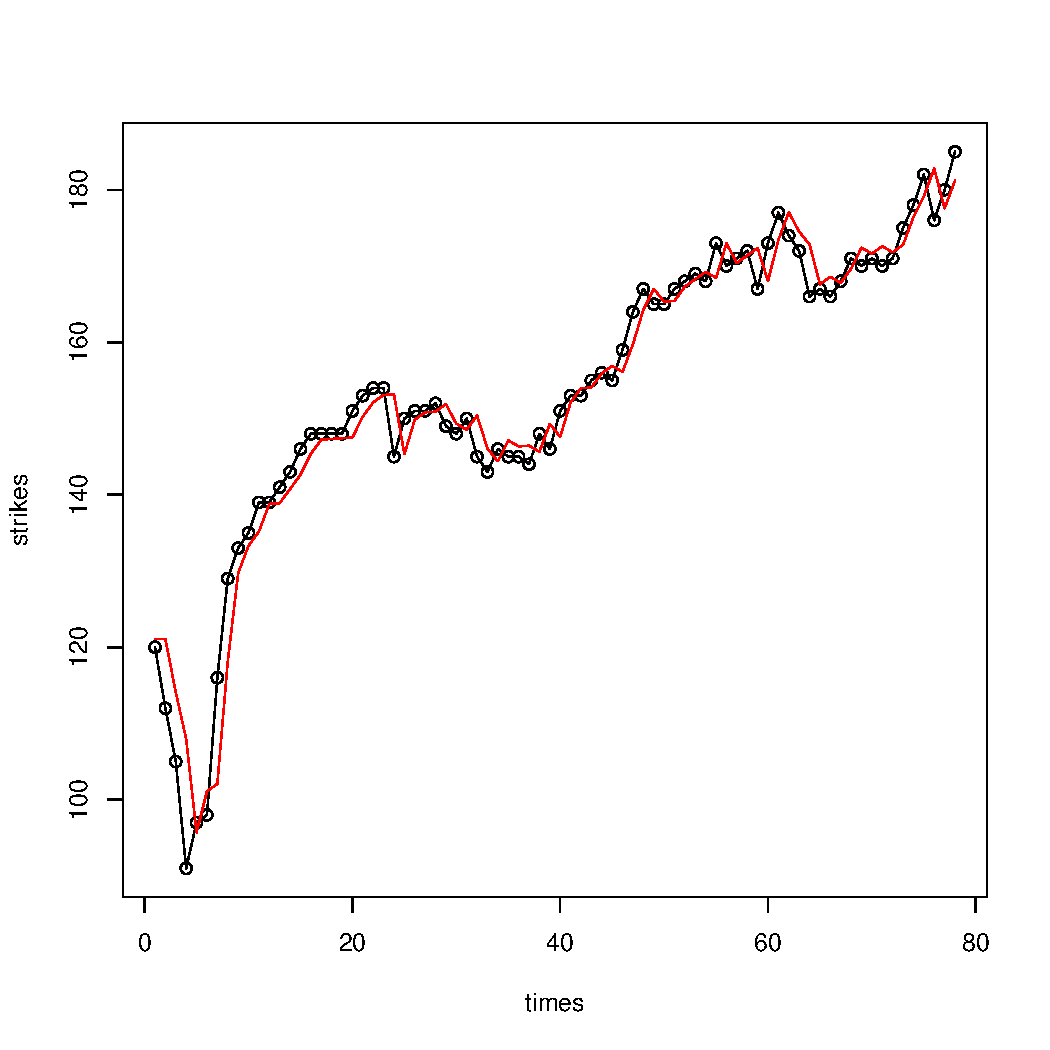
\includegraphics[width=0.6\textwidth]{figs/problem_6/strikes.pdf}
    		\caption{PACF of residuals from linear regression fit.}
    		\label{fig:strikes}
	\end{figure}
	
	\begin{lstlisting}
	
Call:
arima(x = strikes, order = c(1, 0, 0), xreg = times)

Coefficients:
         ar1  intercept   times
      0.8843   121.4793  0.8047
s.e.  0.0485     6.6532  0.1393

sigma^2 estimated as 17.41:  log likelihood = -222.86,  aic = 453.72
	
	\end{lstlisting}
	
	Using the predict() function we find the prediction for the number of strikes in 1981 and find the MSE. 
	
	\begin{lstlisting}
	$pred
	Time Series:
	Start = 79	
	End = 79
	Frequency = 1
	[1] 185.7178

	$se
	Time Series:
	Start = 79	
	End = 79
	Frequency = 1
	[1] 4.172446
	\end{lstlisting}
		
	Our 95\% confidence interval can be constructed as follows 
	
	\begin{equation*}
	P_nX_{n+h}\pm \Phi_{1-\frac{\alpha}{2}}{\sigma_n(h)}
	\end{equation*}
	
	since we assume
	
	\begin{equation*}
	\{{Z_t}\} \sim \text{iid} \ N(0, \sigma^2).
	\end{equation*}
	
	Therefore we calculate or confidence interval as follows
	
	\begin{equation*}
	185.7178 \pm 1.96 \sqrt{17.41}
	\end{equation*}
			
	\end{solution}
	\pagebreak
	
	\begin{problem}{7}
	$ $
	\begin{enumerate}[label=(\alph*)]
		\item Fit a linear regression using ols (lm function in R) and plot the ACF and PACF of the residuals. Are these plots consistent with an AR(1) model?
		\item Fit a linear trend with AR(1) errors to the global temperature data. Use the predict function to predict the next two observations. Show how R is using the coefficients and data to calculate the predictions and use (3.3.19) to verify the calculation of the standard errors for the predictions. 
	\end{enumerate}
	\end{problem}
		
	\begin{solution}{}
	$ $
	\begin{enumerate}[label=(\alph*)]
		\item Figure \ref{fig:temp_ols} shows the linear trend. Observing the ACF and PACF of the residuals, there is evidence to suggest an AR(1) is an appropriate model. There is an exponential decay in the plot of the residuals of the ACF shown in Figure \ref{fig:temp_acf} indicating an AR(1). In addition, the PACF tends toward zero for $h>1$. This also supports our choice of an AR(1). We may question the choice of an AR(1) due to the fact that a number of the lags in the ACF hover above the 1.96 bound. Also lag 6 in the PACF exceeds the bounds.
		
		\begin{figure}[H]
    			\centering
    			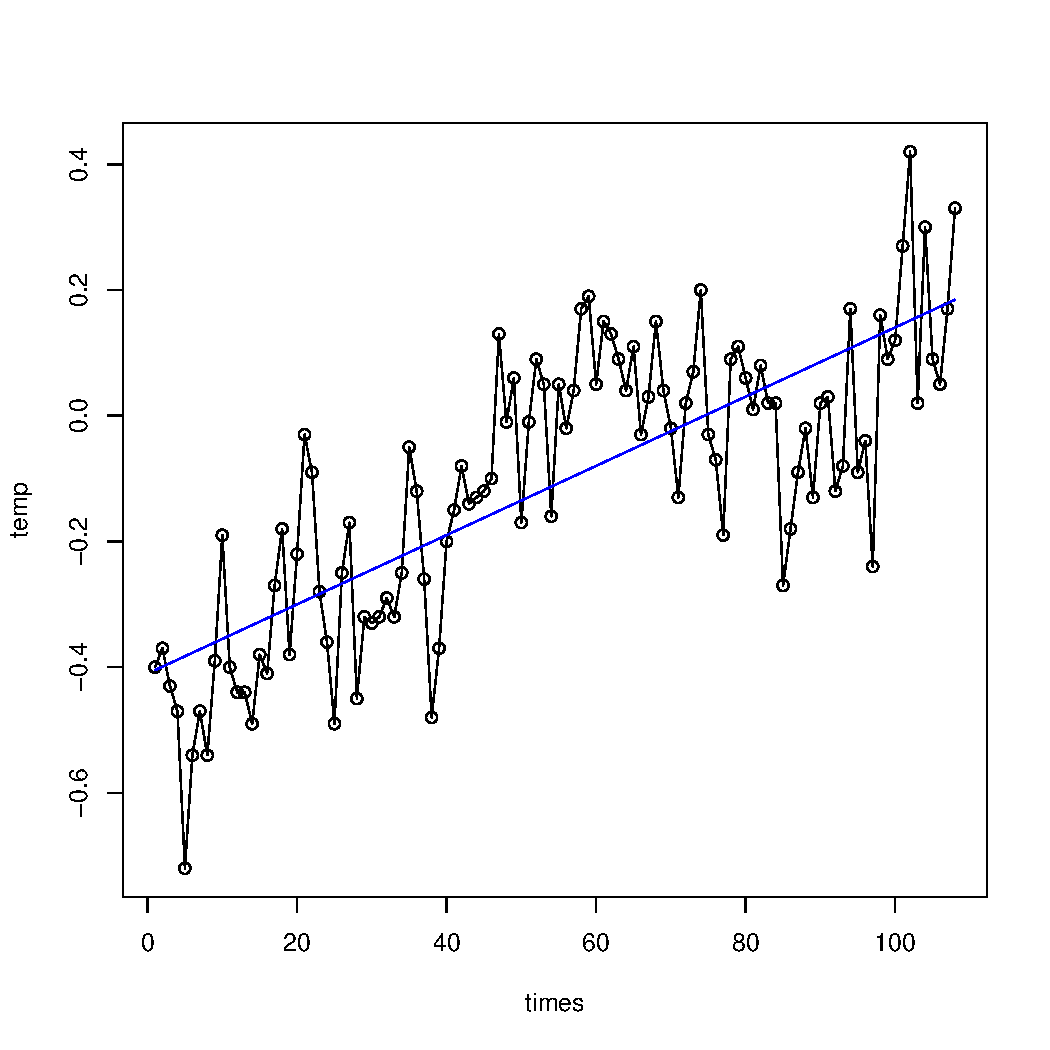
\includegraphics[width=0.6\textwidth]{figs/problem_7/temp_ols.pdf}
    			\caption{Linear regression trend using ols fitted to global temperature data.}
    			\label{fig:temp_ols}
		\end{figure}
		
		\begin{figure}[H]
    			\centering
    			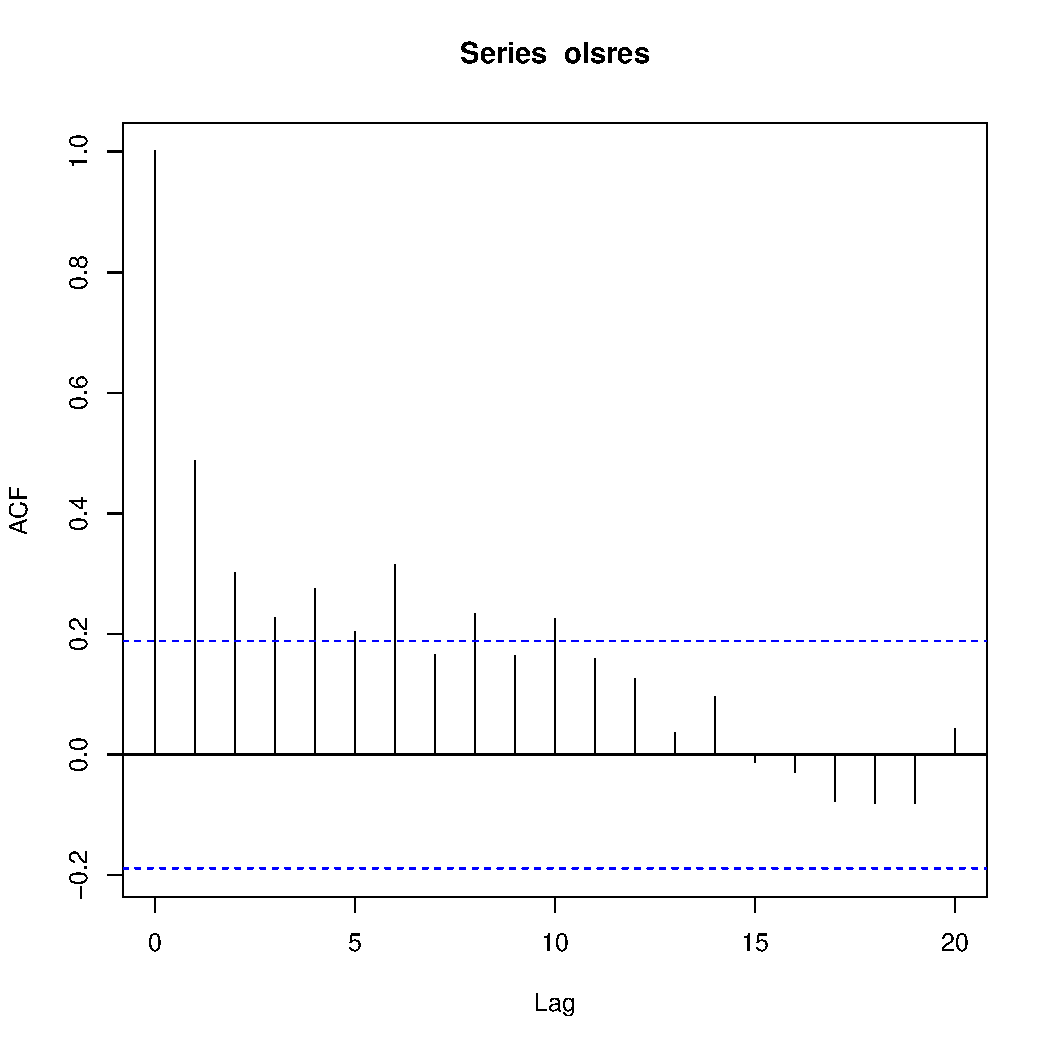
\includegraphics[width=0.6\textwidth]{figs/problem_7/temp_acf.pdf}
    			\caption{ACF of residuals from linear regression fit.}
    			\label{fig:temp_acf}
		\end{figure}

		\begin{figure}[H]
    			\centering
    			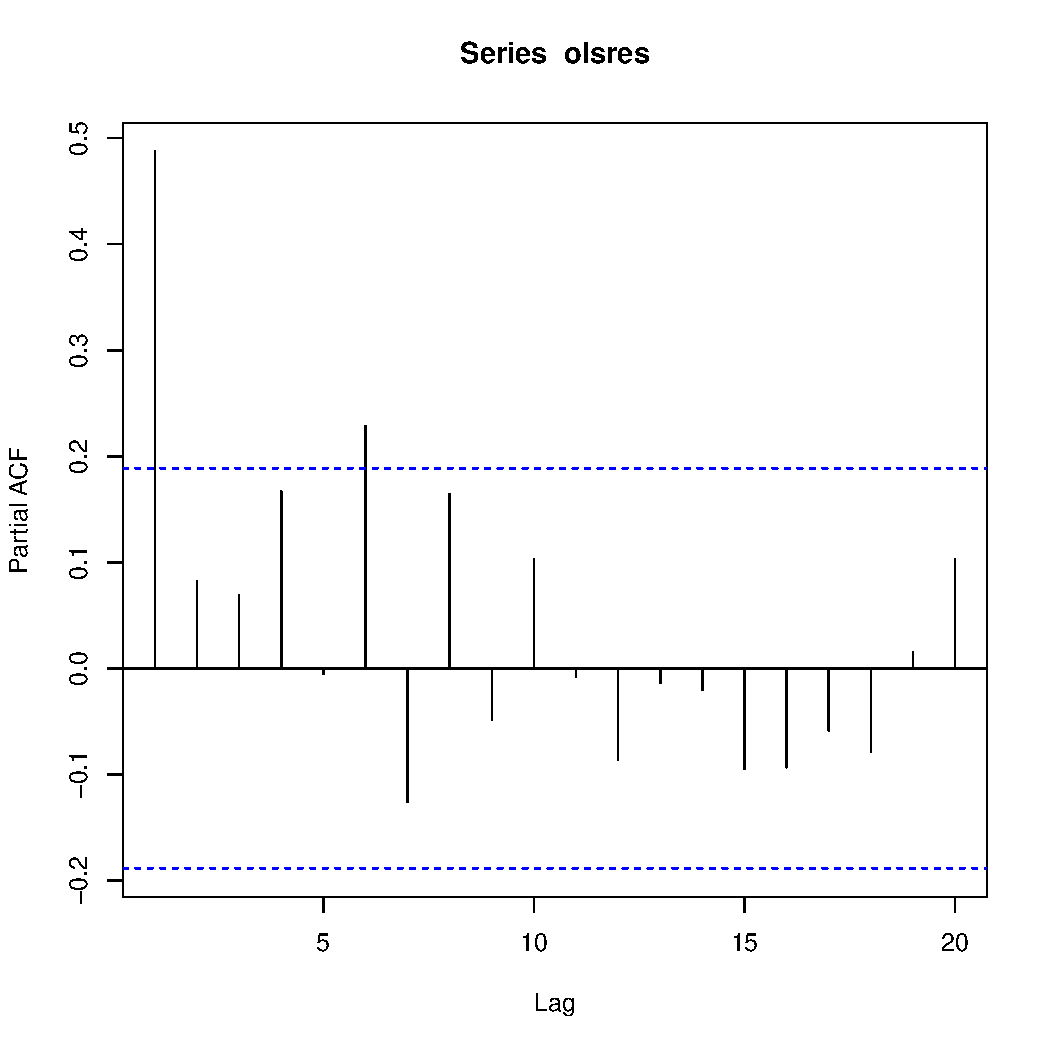
\includegraphics[width=0.6\textwidth]{figs/problem_7/temp_pacf.pdf}
    			\caption{PACF of residuals from linear regression fit.}
    			\label{fig:temp_pacf}
		\end{figure}

		\item Our linear trend with AR(1) errors is shown in Figure \ref{fig:temp_ar1_lin}. The predict() function in R produces the following prediction for the next two time steps.
		
		\begin{lstlisting}
		$pred
		Time Series:
		Start = 109
		End = 110
		Frequency = 1
		[1] 0.2635536 0.2340041
		
		$se
		Time Series:
		Start = 109
		End = 110
		Frequency = 1
		[1] 0.1238722 0.1378180
		\end{lstlisting}
		
		\begin{figure}[H]
    			\centering
    			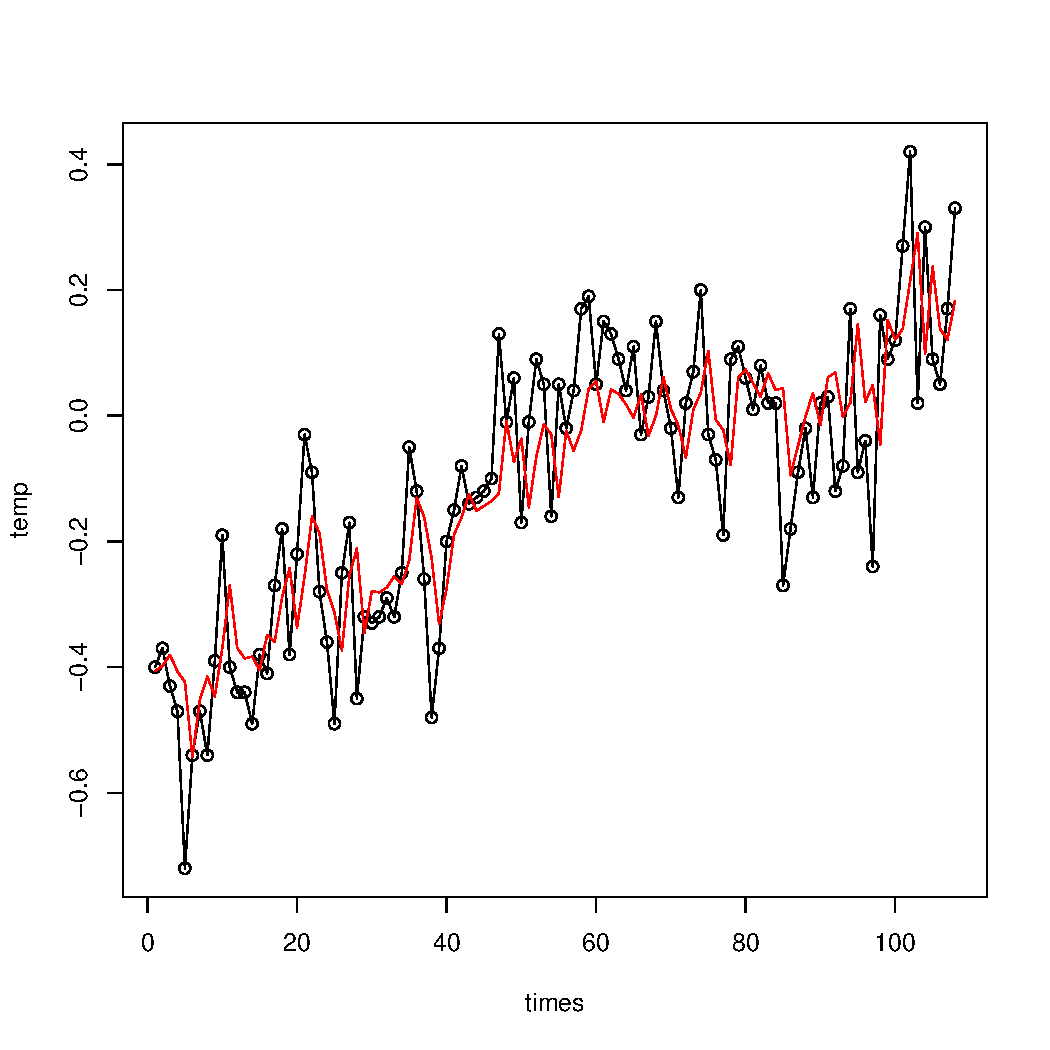
\includegraphics[width=0.6\textwidth]{figs/problem_7/temp_ar1_lin.pdf}
    			\caption{Linear trend with AR(1) errors fitted to the global temperature data..}
    			\label{fig:temp_ar1_lin}
		\end{figure}

		We can check these predictions using the following relationships. 
		
		\begin{align*}
		\hat{X}_{n+1} &= b_o + b_1(n+1) + \hat{\theta}(X_n-b_o-b_1n) \\ 
		\hat{X}_{n+2} &= b_o + b_1(n+2) + \hat{\theta}^2(X_n-b_o-b_1n)
		\end{align*}
		
		Performing this calculation in R as shown below produces the same results as with using the predict() function
		
\begin{lstlisting}[breaklines, frame=single,]
pred1=arfit$coef[2]+(n+1)*arfit$coef[3]+arfit$coef[1]*(temp[n]-arfit$coef[2]-arfit$coef[3]*n)
pred2=arfit$coef[2]+(n+2)*arfit$coef[3]+arfit$coef[1]^2*(temp[n]-arfit$coef[2]-arfit$coef[3]*n)
		\end{lstlisting}
		
		with the results as shown below.
		
		\begin{lstlisting}
		0.2635536
		0.2340041
		\end{lstlisting}
		
		And we can also calculate the standard error using the following relationships
		
		\begin{align*}
		se(\hat{X_{n+1}}) &= \sigma \\
		se(\hat{X_{n+2}}) &= \sigma \sqrt{1 + \phi_1^2}
		\end{align*}
		
		which are derived from (3.3.19)
		
		\begin{equation*}
		\widetilde{\sigma}^2 = \sigma^2 \sum_{j=0}^{h-1} \psi^2_j.
		\end{equation*}
		
		This is implemented in R as follows,
		
		\begin{lstlisting}
		sqrt(arfit$sigma)
		sqrt(arfit$sigma*(1+arfit$coef[1]^2))
		\end{lstlisting}
		
		which produces results that agree with the predict() function.
		
		\begin{lstlisting}
 		0.1238722
		0.137818
		\end{lstlisting}
		
	\end{enumerate}
	\end{solution}
	\pagebreak
	
	\end{document}
	